%%%%%%%%%%%%%%%%%%%%%%%%%%%%%%%%%%%%%%%%%%%%%%%%%%%%%%%%%%%%%%%%%%%%%%%%%%%%%%%%
%2345678901234567890123456789012345678901234567890123456789012345678901234567890
%        1         2         3         4         5         6         7         8

\documentclass[letterpaper, 10 pt, conference]{ieeeconf}  % Comment this line out if you need a4paper

%\documentclass[a4paper, 10pt, conference]{ieeeconf}      % Use this line for a4 paper

\IEEEoverridecommandlockouts                              % This command is only needed if 
                                                          % you want to use the \thanks command

\overrideIEEEmargins                                      % Needed to meet printer requirements.

% See the \addtolength command later in the file to balance the column lengths
% on the last page of the document

% The following packages can be found on http:\\www.ctan.org
\usepackage{graphicx} % for pdf, bitmapped graphics files
%\usepackage{epsfig} % for postscript graphics files
%\usepackage{mathptmx} % assumes new font selection scheme installed
%\usepackage{times} % assumes new font selection scheme installed
\usepackage{amsmath} % assumes amsmath package installed
\usepackage{amssymb}  % assumes amsmath package installed

\title{\LARGE \bf
Efficient Software and Hardware Implementation of the SHA1 Algorithm
}


\author{Justin Cox and Tyler Travis
\\ \small{Deptartment of Electrical and Computer Engineering}
\\ \small{Utah State University}
\\ \small{Logan, Utah 84322}
\\ \small{email: justin.n.cox@gmail.com, tyler.travis@aggiemail.usu.edu}
}


\begin{document}



\maketitle
\thispagestyle{empty}
\pagestyle{empty}


%%%%%%%%%%%%%%%%%%%%%%%%%%%%%%%%%%%%%%%%%%%%%%%%%%%%%%%%%%%%%%%%%%%%%%%%%%%%%%%%
\begin{abstract}

This paper describes the process of implementing fast and efficient password-cracking devices.  The hashing algorithm that this paper will consider is the SHA1 algorithm.  X86-64 and FPGA password-cracking implementations were designed and analyzed to measure the speed and throughput of each design.

\emph{Index Terms}---Passwords, SHA1, password-cracking, security,  authentication.    

\end{abstract}

%%%%%%%%%%%%%%%%%%%%%%%%%%%%%%%%%%%%%%%%%%%%%%%%%%%%%%%%%%%%%%%%%%%%%%%%%%%%%%%%
\section{INTRODUCTION}

There are several methods of securely storing data such as encryption and hashing.  For this paper we will focus on the latter, more specifically, we will focus on the SHA1 algorithm of a hash.

Since a hash is defined as a one way function, it is almost impossible to find the original message given the hash of the message.  In an application such as password recovery, it is important that we can generate hashes quickly so that we can compare the hash of a known message with the hash of an unknown message.

This paper will describe two implementations of the SHA1 algorithm that were specifically designed with the hardware architecture in mind to increase the throughput of the design.

\subsection{SHA1 Algorithm Overview}

To help the reader better understand the optimizations that are later discussed in the paper, the authors thought it necessary to give a brief overview of how the SHA1 algorithm is implemented.

The SHA1 algorithm is similar to the MD5 algorithm invented by Ronald L. Rivest.  The SHA1 algorithm is able to take any message of size $n$ and splits that message into 512-bit chunks.  The last chunk will be padded starting with a bit 1 and will be padded with bits 0 until the size of the last chunk is 448 mod 512.  The last 64 bits will be used to append the size of the original message in bits.

The message is then split into 16, 32-bit words.  These 32-bit words are then used to expand the original 512-bit chunk by 2048 more bits.  The now 80, 32-bit words are operated on to produce a hash.  If the message has more than one 512-bit chunk, the produced hash will be passed into the next hashing function as the input and a new 512-bit chunk will be fed into the hashing function.  The operations performed on the 80, 32-bit words are illustrated in Figure 1.

\begin{figure}[thpb]
	\centering
	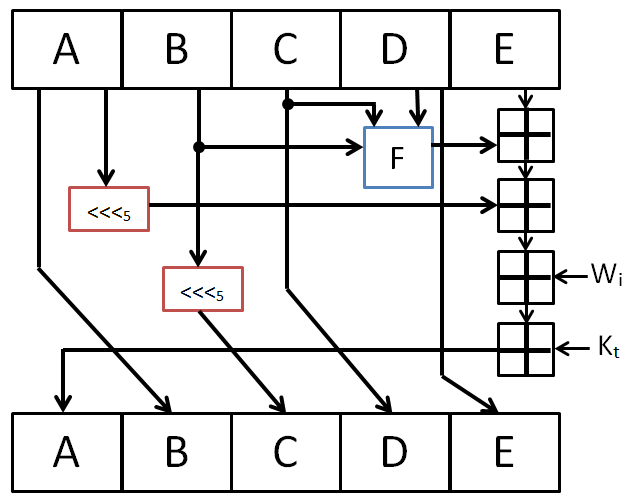
\includegraphics[scale=0.5]{sha1}
    \caption{A flowchart of one iteration within the SHA1 compression function where blocks $A,B,C,$ and $D$ are 32-bit words.}
\end{figure}

This paper will not cover more details about the SHA1 algorithm, but the authors encourage the reader to learn more about it from other resources available. 

\section{SOFTWARE IMPLEMENTATION}

The language chosen for the software implementation of the SHA1 algorithm is C.  This section will describe optimizations chosen by the authors beginning with code structure optimizations and finishing with architecture-aware optimizations.

\subsection{Loop Unrolling}

Loop unrolling is a well known technique used to minimize unnecessary overhead due to loop instructions.  Since SHA1 is a well-defined, sequential algorithm, we are able to unroll all of the loops because the size of the iterations is known.  We were able to see an improvement in the speed of the hash generation.  More detailed results will be given in the $Results$ section.   

\subsection{User-Defined MACROS}

A macro is a single user-defined instruction that is used to carry out multiple instructions.  Compiler-defined macros in C actually replace the macro with the desired code at compile time.  There are many routines which are executed often in the SHA1 algorithm.  Normally, programmers would opt to create a function to improve the readability of the code and to decrease the programmer's time needed to write the algorithm.  However with function calls, comes more overhead.  A macro will provide readable code while also eliminating function call overhead.

The authors were able to notice that the SHA1 compression algorithm uses many left rotate operations by different shifting amounts.  The authors tested a function implementation and compared it to a macro implementation.  The macro implementation, on average, had a $15$ to $20\%$ increase in efficiency.     

\subsection{SHA1 Algorithm Exploit}

In 2011, Jens Steube was able to exploit a weakness found in the SHA1 algorithm. He claims that he is able to optimize the instruction count by $21.1\%$ [1].  The authors desired to learn more about the exploit and to see if the results from Jens Steube could be validated and replicated.

A quick explanation, the weakness is due to the properties of the XOR operation.  Since a logical operation such as XOR cannot overflow, we can use this to our advantage.  In order to make this exploit work, the password generator has to create the password candidates in a specific way.  If the 512-bit chunks are made up of 16, 32-bit words defined as $w[0],w[1]...w[15]$, the password generator must keep $w[1] \-- w[15]$ constant while $w[0]$ iterates through the defined character set as shown in Figure 2.

\begin{figure}[thpb]
	\centering
	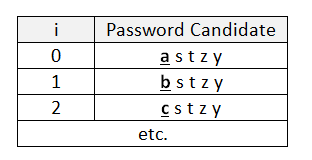
\includegraphics[scale=.75]{passwordGeneration}
    \caption{An example table that shows how the password generation must generate passwords.}
\end{figure}

If password candidates are generated in this manner, we are able to pre-compute words $w[1]\--w[15]$ and the expansion words $w^{'}[16]\--w^{'}[79]$.  We then only have to compute $w[16]\--w[79]$ by XORing with the dynamic variable $w[0]$.  An example is given as follows:


$$w[16] = w^{'}[16]\ XOR\ w[0]\_1$$
$$w[17] = w^{'}[17]$$
$$w[18] = w^{'}[18]$$
$$w[19] = w^{'}[19]\ XOR\ w[0]\_2$$

\noindent
where the $\_1$ and $\_2$ denote the amount that $w[0]$ needs to be left rotated by.

We did not look at the assembly of the code to validate and check the  optimization of the number of instructions, but the program was run to test for an increase in efficiency.  We were able to observe a $15$ to $20\%$ increase in efficiency on our machine.
   
\subsection{SIMD}

Single Instruction Multiple Data (SIMD) is a feature provided by modern day processors to be able to compute operations on multiple data for the cost of a single instruction.  Specifically, our program uses SIMD features provided by Intel's Advanced Vector Extensions (AVX). AVX is a new set of high performance instructions similar to Intel's Streaming SIMD Extensions (SSE).  AVX introduced operations performed on 256-bit vector registers compared to the 128-bit registers of SSE.  It also introduced other features such as a more effecient way to store results from vector operations.  Instead of $A = A + B$, it is possible to compute $C = A + B$ which preserves vector $A$ and $B$ limiting memory read and writes.  Unfortunately, AVX1 only does floating point operations using the 256-bit registers and the SHA1 algorithm works with integers.  Integer operations using 256-bit registers are implemented in AVX2 [2].

The AVX registers in our program are used to be able to compute four hashes in parallel.  In the SHA1 compression iteration four, 32-bit words $a0, a1, a2, a3$ are stored into vector $A$, $b0, b1, b2, b3$ are stored into vector $B$, and so on.  We also make use of the $\_mm\_andnot\_si128()$ Intel Intrinsic function which eliminates one instruction.  Although the program is limited to using SSE Intrinsic instructions, the authors chose to use AVX to take advantage of AVX's ability to preserve registers.  The functions in the SHA1 compression algorithm re-use the same vectors multiple times.  Without the register preserve functionality of AVX, the program would receive a greater memory penalty.  

\subsection{Parallel Computing}

The password generation section of the code is written so it generates and checks four passwords at once.  We were able to notice a significant improvement than the single password generator.

The authors also took advantage of the $pthreads$ library in C.  Two different threads were implemented to split up the password candidate space in half to increase the operation speed. 

\subsection{Results}

To test our SHA1 password-cracker, we were given an unknown hash of bd38 849c eb2b dfe7 312d 3d27 2483 8f2b 9b09 c724.  After running the unknown hash, we were able to retrieve the password of "HeyHey".

After benchmarking our code with the previously discussed optimizations, we were able to come up with the following results:

\begin{center}
    \begin{tabular}{| p{4cm} | l |}
        \hline
         Optimization & Million Hashes per Second \\ \hline
        Baseline (AVX + Loop Unrolling) & .73 \\ \hline
        Optimization 1 (Baseline + XOR exploit) & 3.45 \\ \hline
        Optimization 2 (Baseline + pthreads) & .80 \\ \hline
        Combined Optimization & .87 \\
        \hline
    \end{tabular}
\end{center}

\noindent
\\
The baseline implementation combined with the XOR exploit had the greatest results.  The multi-threaded version had slightly better results on average but sometimes it had worse results than the baseline.  Since the multi-threads split the candidate space in half, better efficiency is achieved if the password is located close to the thread's initial starting points.

\section{HARDWARE IMPLEMENTATION}

Based on the results of the software implementation, the SHA1 hashing algorithm does take some time to generate the results.  The paper will now discuss a hardware dedicated implementation of the SHA1 hash generation.  The FPGA used for the implementation is a Digilent BASYS 2 board.
\subsection{Architecture}

The authors decided to design a fully unrolled implementation of the system.  This decision was made so that a pipelined version could be easily added in the future.  The inputs to each round are $A$, $B$, $C$, $D$, $E$, $K$, $W$, and $CLK$.  The outputs to each round are $AOUT$, $BOUT$, $COUT$, $DOUT$, and $EOUT$.  Each round is comprised of 20 different iterations.  If there is not a lot of overhead in the design, this implementation should take around 80 cycles to compute a hash.

\subsection{Benchmarking Results}

The performance of the FPGA implementation was calculated using the following formula:

$$
Throughput = \frac{Block\ Size * Clock\ Frequency}{Cycles\ per\ Block}\eqno{(1)} 
$$

\noindent
The block size is 512 (512-bits * 1 SHA1). The Clock frequency was set to the external oscillator of the FPGA of 50MHz.  The hash is produced in 93 cycles.  Using these numbers we come up with

$$Throughput = \frac{512*50,000,000}{93} \approx 27.5Mhps$$

\noindent
or 27.5 Mega hashes per second.  These results were verified in hardware in Figure 3 using an oscilloscope.

We can see that the FPGA implementation generates better results then the software implementation.  This number could be improved if a fully unrolled, pipelined version was developed.  Furthermore, according to the timing report given in Xilinx, we are able to increase the clock frequency but the authors chose to use the external oscillator of 50MHz.

\begin{figure}[thpb]
	\centering
	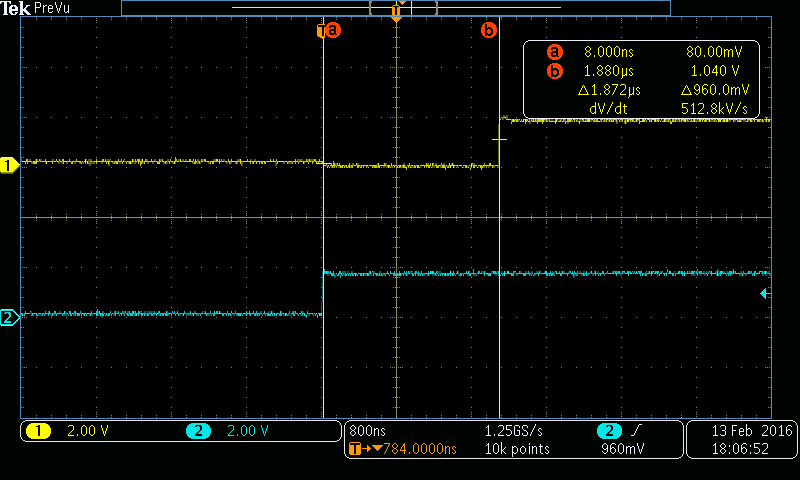
\includegraphics[scale=.35]{tek00001}
    \caption{The blue signal is when the program initiates. The yellow signal is when the hash has been computed and verified.}
\end{figure} 


\section{CONCLUSION}

This paper gives an example of how software optimization and hardware implementations can improve the amount of hashes a password-cracker can compare.  It is important to understand the architecture of the hardware the program is being run on to fully take advantage of the speed available.

From a security perspective, it is better for a hash algorithm to take a long time to ensure that a password-cracker will not have enough time to guess the desired password.  From a hacker's perspective, the quicker you can make your hashing algorithm, the more passwords you will be able to recover.

\addtolength{\textheight}{-12cm}   % This command serves to balance the column lengths
                                  % on the last page of the document manually. It shortens
                                  % the textheight of the last page by a suitable amount.
                                  % This command does not take effect until the next page
                                  % so it should come on the page before the last. Make
                                  % sure that you do not shorten the textheight too much.

%%%%%%%%%%%%%%%%%%%%%%%%%%%%%%%%%%%%%%%%%%%%%%%%%%%%%%%%%%%%%%%%%%%%%%%%%%%%%%%%



%%%%%%%%%%%%%%%%%%%%%%%%%%%%%%%%%%%%%%%%%%%%%%%%%%%%%%%%%%%%%%%%%%%%%%%%%%%%%%%%



%%%%%%%%%%%%%%%%%%%%%%%%%%%%%%%%%%%%%%%%%%%%%%%%%%%%%%%%%%%%%%%%%%%%%%%%%%%%%%%%

%\section*{ACKNOWLEDGMENT}

%The author would like to thank his instructor Dr. Rajnikant Sharma %for his help in understanding control concepts.




%%%%%%%%%%%%%%%%%%%%%%%%%%%%%%%%%%%%%%%%%%%%%%%%%%%%%%%%%%%%%%%%%%%%%%%%%%%%%%%%




\begin{thebibliography}{99}

\bibitem{c1} Steube, Jens. (2012, Nov. 20). \emph{Exploiting a SHA1 Weakness In Password Cracking}[Online]. Available: http://hashcat.net/events/p12/
\bibitem{c2} Lomont, Chris. (2011, June 21). \emph{Introduction to Intel Advanced Vector Extensions}[Online]. Available: https://software.intel.com/en-us/articles/introduction-to-intel-advanced-vector-extensions
 

\end{thebibliography}

\begin{figure}[thpb]
	\centering
	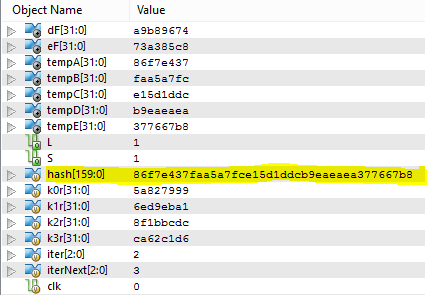
\includegraphics[scale=.75]{hash}
    \caption{Verification of the hash of password "a" in FPGA Simulation.}
\end{figure}


\end{document}
